\documentclass[twocolumn]{article}
\usepackage[margin=0.6in,columnsep=0.15in]{geometry}
\usepackage[utf8]{inputenc}
\usepackage{stix}
\usepackage{microtype}
\usepackage[usenames,dvipsnames]{color}
\usepackage[colorlinks,citecolor=Gray,urlcolor=Gray,linkcolor=Cyan]{hyperref}

\usepackage{abstract}
\setlength{\absleftindent}{1in}
\setlength{\absrightindent}{\absleftindent}

\usepackage{authblk}
\renewcommand\Affilfont{\itshape\small} % chktex 6

\usepackage[normal]{caption}
\DeclareCaptionLabelSeparator{pipe}{ $|$ }
\captionsetup{labelsep=pipe}
\renewcommand{\captionfont}{\small}
\renewcommand{\captionlabelfont}{\bfseries}

\usepackage[comma,sort&compress]{natbib}
\usepackage{natmove}
\bibliographystyle{achemso}
\renewcommand\cite{\citep}
\AtBeginDocument{\nocite{achemso-control}}

\newcommand\doi[1]{\href{http://dx.doi.org/#1}{\nolinkurl{#1}}}

\usepackage{graphicx}
\usepackage{mathtools}
\usepackage{booktabs}
\usepackage{tabularx}
\usepackage[export]{adjustbox}

\title{On the range of electron correlation in density functional theory: Supplementary information}

\author[1]{Jan Hermann}
\author[1]{Matthias Scheffler}
\author[2,*]{Alexandre Tkatchenko}
\affil[1]{Fritz-Haber-Institut der Max-Planck-Gesellschaft, Faradayweg 4--6, 14195 Berlin, Germany}
\affil[2]{Physics and Materials Science Research Unit, University of Luxembourg, 162A Avenue de la Faïencerie, L-1511 Luxembourg}
\affil[*]{\normalfont{Email: alexandre.tkatchenko@uni.lu}}

\date{}

\setcounter{secnumdepth}{0}

\begin{document}

\begin{figure*}
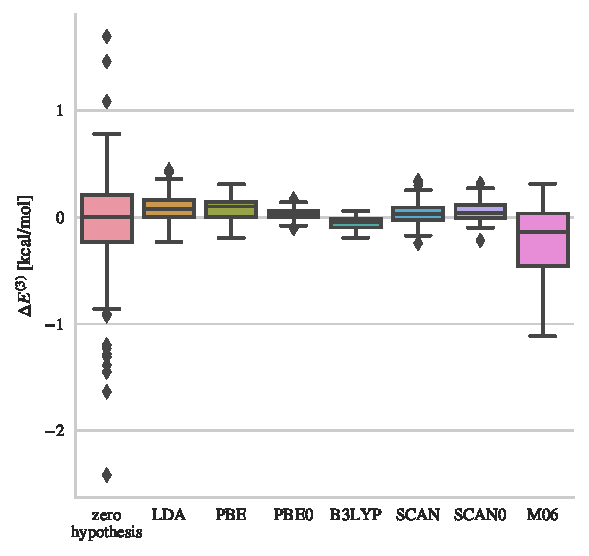
\includegraphics[center]{../media/3-body}
\caption{\textbf{Label.}
Text.
\label{fig:3-body}
}
\end{figure*}

\begin{figure*}
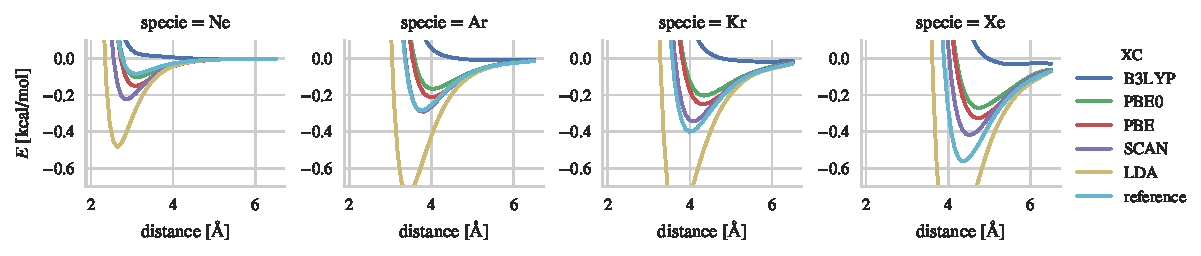
\includegraphics[center]{../media/mbd-rare-gas}
\caption{\textbf{Label.}
Text.
\label{fig:mbd-rare-gas}
}
\end{figure*}

\begin{figure*}
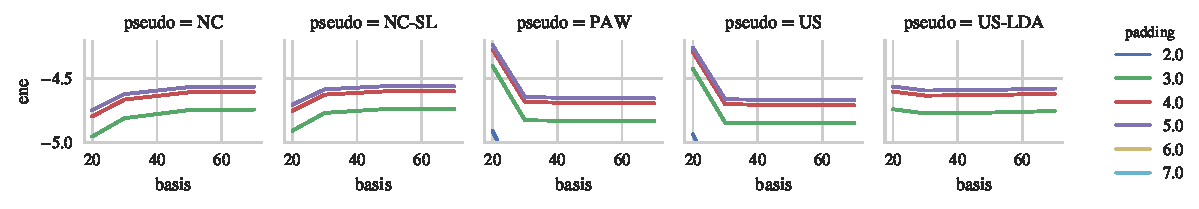
\includegraphics[center]{../media/bz-tests-padding-basis}
\caption{\textbf{Label.}
Text.
\label{fig:bz-tests-padding-basis}
}
\end{figure*}

\subsubsection{Supplementary References}

\begingroup
\renewcommand{\section}[2]{}%
\bibliography{achemso,suppl}
\endgroup

\end{document}
